\chapter{Digitializing the Cube}
\myTop{In order to implement solving algorithms on a Rubik's Cube the cube itself must first be digitialized and a visual interface must be created in order to see the result of any algorithm. In this chapter the process of getting the Rubik's Cube into the computer is described.}
A \rubik{} is a rather complicated 3-dimensional structure and fitting this structure into a computer system is quite complicated. 
The \rubik{} is build up by 26 \cpiece{}s held together by each other. 
This type of structure is not straight forward to implement into a computer. If the \rubik{} is depicted in the computer in a two-dimensional space, its depiction will be far from the original \rubik{} structure.

A simple way to handle the \rubik{} in the program is a two dimensional depiction and  just simply move the \facelet{}s around.
The analogue to this on a real \rubik{} will be to take of the the colored stickers and move them to their new position rather than actually move the \cubie{}s when one is to make a twist of the \rubik{}.
This approach will be far from reality and will make the implementations of solving algorithms, such as Kociembas optimal solver more complicated, since it will be harder for the algortihm to determine the place of the \cpiece{}s.

An object-oriented approach to the problem will give a more useful structure. 
Dividing the \rubik{} into its sub structures. 
The cube consist of the 6 faces each with 9 shared \cpiece{}. 
A face also consist of 9 \cubicle{}s which acts as placeholders for the \cpiece{}s. 
There are 3 types of \cpiece{} and cubicles; corner, edge and centers. 
The center \cpiece{}s will never move and therefore there are no reason to define a \cubicle{} and a \cpiece{} for those. Instead the face is simple granted a \facelet{} which defines the color of the given face.
\begin{figure}[h]
	\centering
		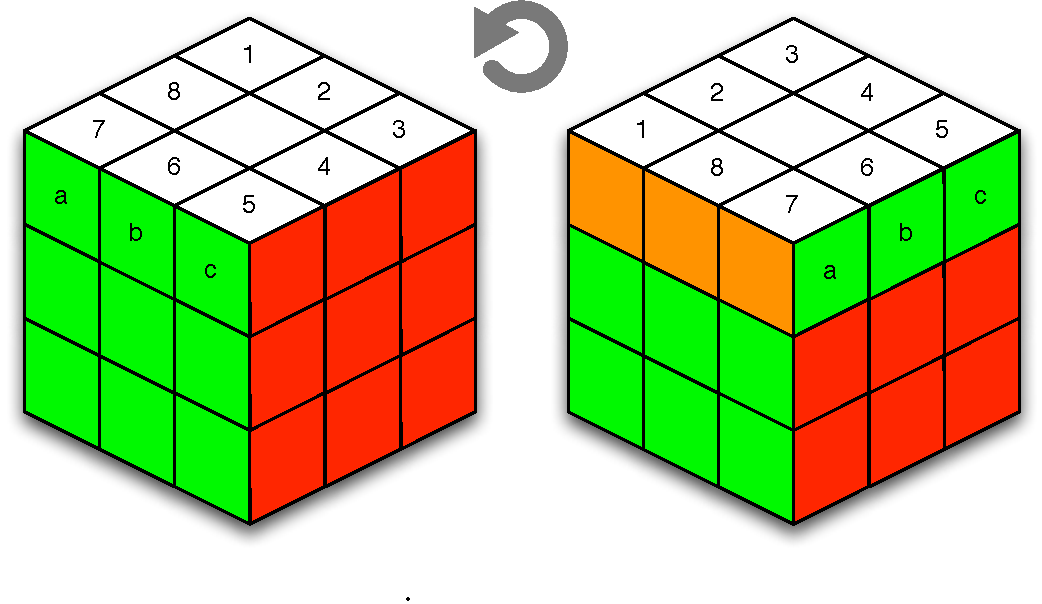
\includegraphics[scale=0.6]{input/pics/twistOfUpFace.pdf}
	\caption{\myCaption{A twist of a face will not only inflict the twisted face but also its adjacent faces. }}
	\label{fig:twistOfUpFace}
\end{figure}
This structure allows for the same \cubicle{} to be in several faces. 
Two faces for edges and three for corners. 
In this structure moving a face will move the \cpiece{}s around in the \cubicle{}s. See figure \ref{fig:twistOfUpFace}.This makes the adjacent face to the moving face, get some of its \cpiece{}s moved to other \cubicle{}s as well. 
For example when twisting the up face of a \rubik{} will inflict the move the \cpiece{}s of the R, L, B and F faces. 

The problem of this structure though is it requires variables to determined how the \facelet{} should be orientated. 
How this is done is described in chapter ref\{Somewhere\}.
